%!TEX root = ../dissertation.tex
\pagestyle{empty}
\null
\newpage
%\thispagestyle{empty}

\vspace*{\fill}

\begin{center}
	%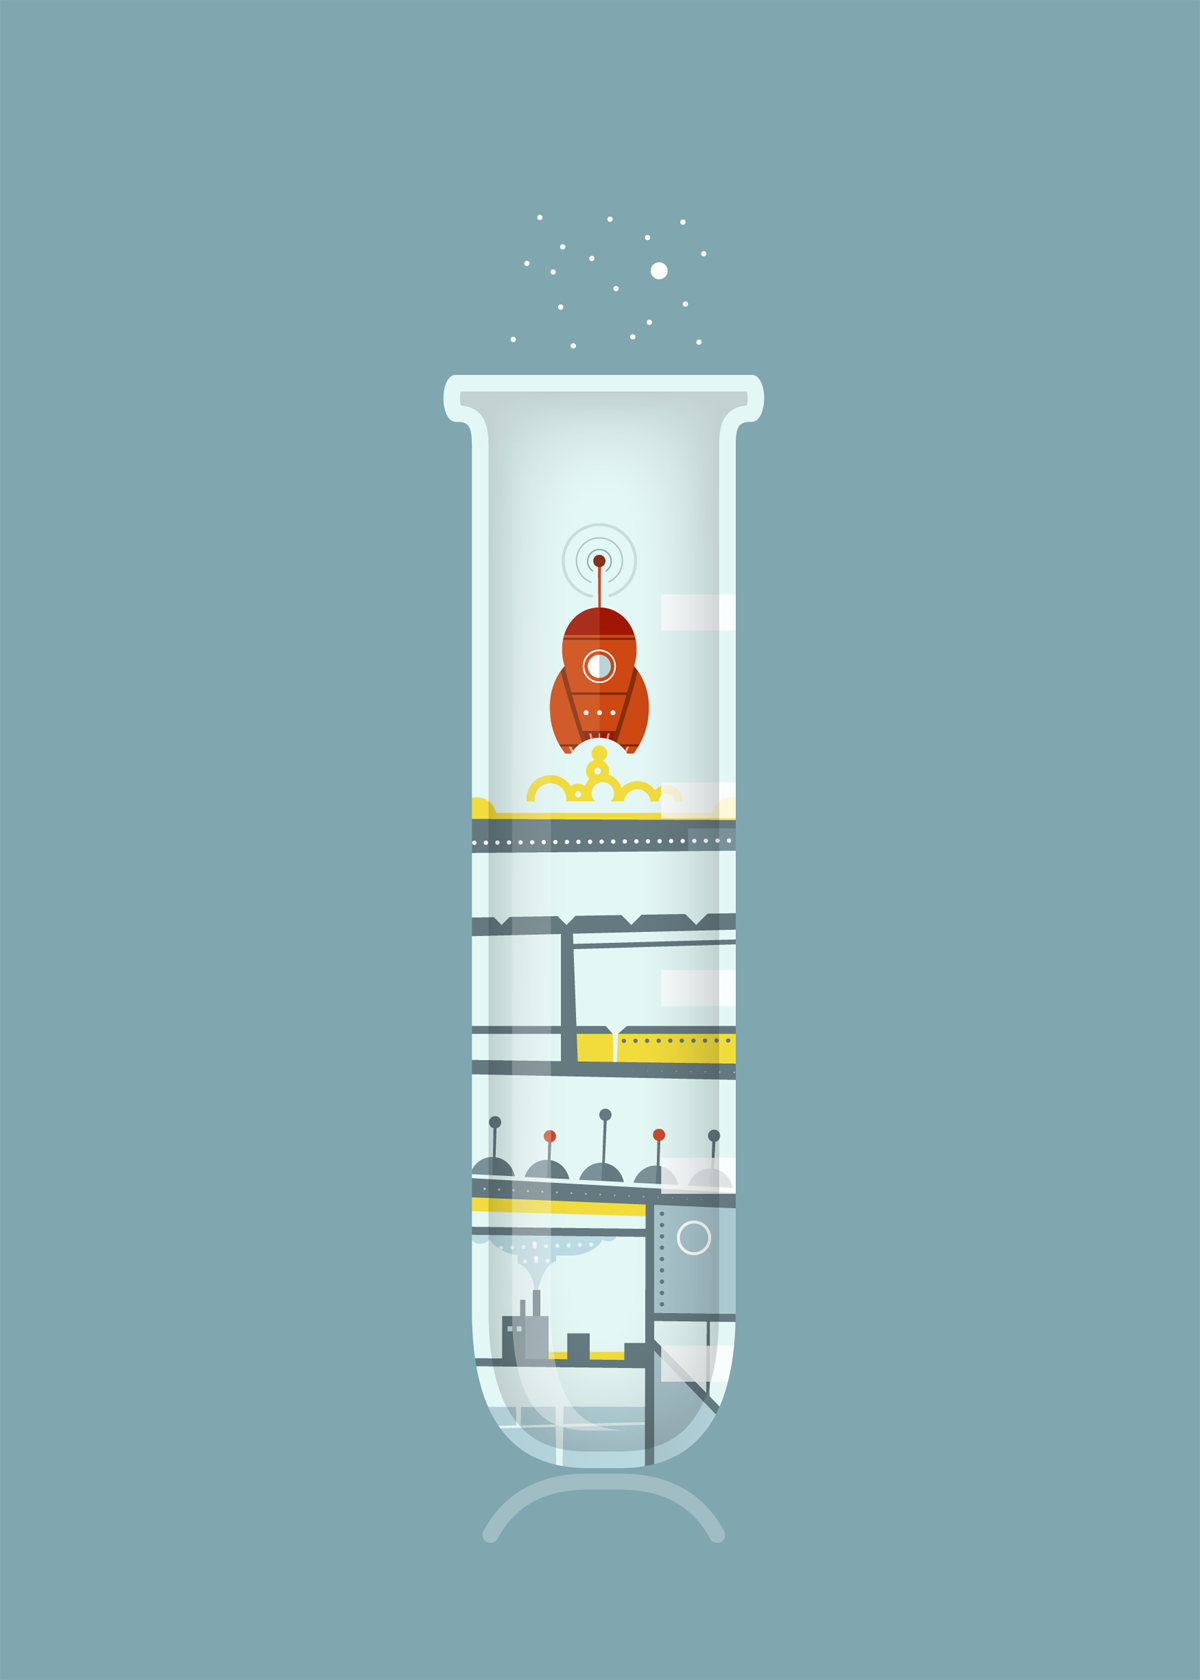
\includegraphics[width=0.42\textwidth]{endmatter/colophon.png}
	
	%\vspace{30pt}
	
	\parbox{0.7\textwidth}{
		\lettrine[lines = 3, loversize = -0.1, lraise = 0.1]{\textcolor{school_red}{Q}}{uesta tesi} è stata scritta usando \LaTeX, originariamente sviluppato da Leslie Lamport e basato sul \TeX di Donald Knuth.
		Il testo del corpo è riportato in 12 punti MinionPro, basato sull'omonimo Minion disegnato da Robert Slimbach e ispirato allo stile tardo-rinascimentale; il carattere è stato progettato per il corpo del testo in uno stile classico, leggermente condensato e con grandi aperture per aumentare la leggibilità.
	}
	
	\vspace{3em}
	
	%Finita di stampare il \today.
\end{center}